\chapter{Development environment}

In this chapter the environment of the development will be described, where the structure of the vehicle and its sensors, and the requirements of the estimator will be discussed.

\section{Available sensor data}

A modern vehicle is equipped with multiple ECU-s, numerous sensors and actuators that support and enhance driving quality. When considering vehicle motion control applications the mostly used and available sensors are the following:
\begin{table}[ht]
\centering
\begin{tabular}{|c|c|c|}
\hline
\textbf{Sensor Type} & \textbf{Variables} & \textbf{Unit of Measurement} \\
\hline
Wheel speed sensor & $\omega_{FR}, \omega_{FL}, \omega_{RR}, \omega_{RL}$ & [$^\circ$/s] \\
\hline
Wheel torque sensor & $M_{FR}, M_{FL}, M_{RR}, M_{RL}$ & [Nm] \\
\hline
Acceleration from IMU & $a_x$, $a_y$, $a_z$ & [m/s$^2$] \\
\hline
Angular rates from IMU & $\dot{\alpha}$, $\dot{\beta}$, $\dot{\gamma}$ & [$^\circ$/s] \\
\hline
Brake pressure sensor & $P_{FR}, P_{FL}, P_{RR}, P_{RL}$ & [bar] \\
\hline
Road wheel angles & $\delta_{FR}, \delta_{FL}, \delta_{RR}, \delta_{RL}$ & [$^\circ$] \\
\hline
Steering wheel angle & $\varphi$ & [$^\circ$] \\
\hline
\end{tabular}
\caption{Overview of sensor types, variables, and units}
\label{tab:sensor_table}
\end{table}


GNSS receivers can be also considered as precise sensors that are available during the development phase but not on the vehicles from the production line in order to keep the wider availability. Therefore the calculated longitudinal and lateral speeds from the GNSS measurements will only serve for reference, validation, testing and training purposes. The mentioned sensor units can be seen on figure \ref{fig:sensors}. 

\FloatBarrier
\begin{figure}[ht]
    \centering
    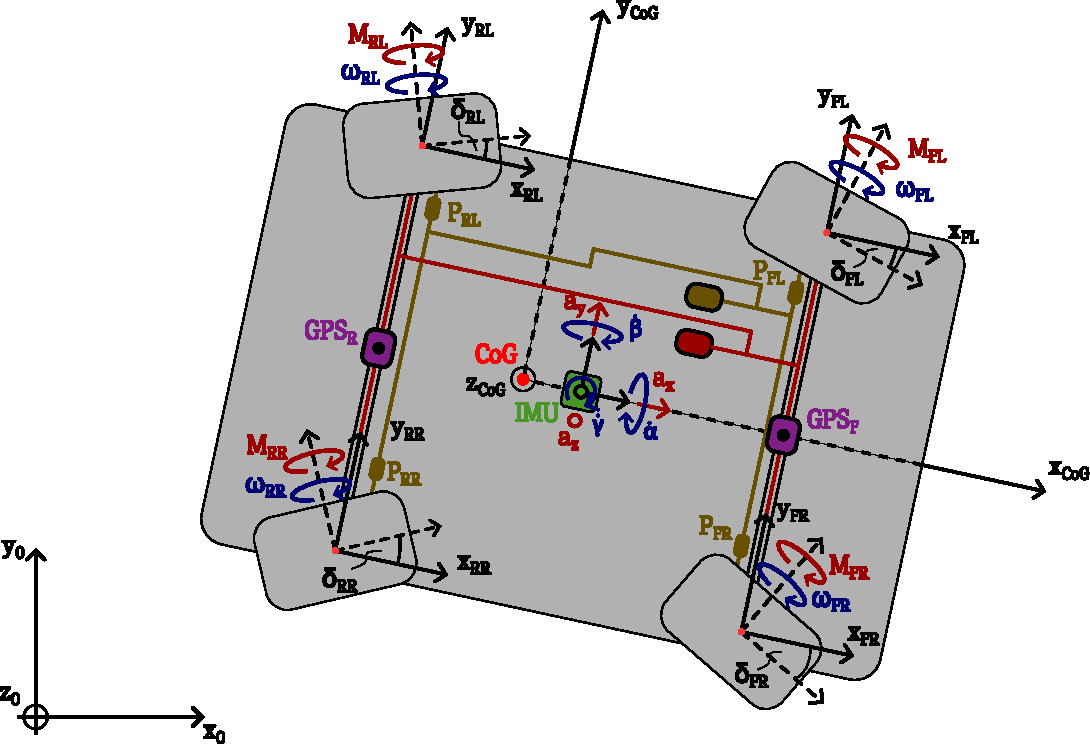
\includegraphics[width=1\textwidth]{images/sensors.pdf}
    \caption{Available sensor data for speed estimation}
    \label{fig:sensors}
\end{figure}
\FloatBarrier

The structure of the available sensor on the CAN bus data that was used in the further development is the following. Sampling time is 2 [$ms$] for all the sensors except the speed values provided by the GNSS receivers, that is 100 [$ms$]. Above this, the sensor data is collected in a large enough buffer to provide all the values at the same time. This way at every 2 [$ms$] all the inputs will arrive at the same time to the estimator. The speeds from the GNSS receivers will be handled separately from base structure. The structure can be seen in table \ref{tab:data_structure}:

\FloatBarrier
\begin{table}[htbp]
\centering
\resizebox{\textwidth}{!}{%
\begin{tabular}{|c|c|c|c|c|c|c|c|c|c|c|c|c|c|c|c|}
\hline
\textbf{time} & $a_x$ & $\omega_{FR}$ & $\omega_{FL}$ & $\omega_{RR}$ & $\omega_{RL}$ & $M_{FR}$ & $M_{FL}$ & $M_{RR}$ & $M_{RL}$ &  $a_y$ & $a_z$ & $\dot\alpha$ & $\dot\beta$ & $\dot\gamma$ & ...\\ \hline
$\vdots$ & $\vdots$ & $\vdots$ & $\vdots$ & $\vdots$ & $\vdots$ & $\vdots$ & $\vdots$ & $\vdots$ & $\vdots$ & $\vdots$ & $\vdots$ & $\vdots$ & $\vdots$ & $\vdots$ & ...\\ \hline
6.220&0.2819&31.3643&31.3791&31.5755&31.5894&0&0&19.087&19.087&0&0&0&0&0.2329&...\\ \hline
6.222&0.2819&31.3643&31.3791&31.5755&31.5894&0&0&19.087&19.087&0&0&0&0&0.2349&...\\ \hline
6.224&0.2819&31.3643&31.3791&31.5755&31.5894&0&0&19.087&19.087&0&0&0&0&0.2369&...\\ \hline
6.226&0.2819&31.3643&31.3791&31.5755&31.5894&0&0&19.087&19.087&0&0&0&0&0.2389&...\\ \hline
6.228&0.2819&31.3643&31.3791&31.5755&31.5894&0&0&19.087&19.087&0&0&0&0&0.2409&...\\ \hline
6.230&0.2893&31.511&31.5304&31.7222&31.7406&0&0&19.087&19.087&0&0&0&0&0.2429&...\\ \hline
6.232&0.2893&31.511&31.5304&31.7222&31.7406&0&0&19.087&19.087&0&0&0&0&0.2449&...\\ \hline
6.234&0.2893&31.511&31.5304&31.7222&31.7406&0&0&19.087&19.087&0&0&0&0&0.2469&...\\ \hline
$\vdots$ & $\vdots$ & $\vdots$ & $\vdots$ & $\vdots$ & $\vdots$ & $\vdots$ & $\vdots$ & $\vdots$ & $\vdots$ & $\vdots$ & $\vdots$ & $\vdots$ & $\vdots$ & $\vdots$ & ...\\ \hline
\end{tabular}%
}
\caption{Example of available data structure with 2[$ms$] sampling time}
\label{tab:data_structure}
\end{table}
\FloatBarrier

\section{Ways to use AI to estimate vehicle speed}

Before advancing to the possible algorithms for vehicle speed estimation using AI, some high level requirements shall be set to be able to validate the results. The requirements are the following:
\begin{enumerate}
    \item The developed estimator shall provide more accurate vehicle speed values than a model based vehicle speed estimator.
    \item The developed estimator shall be tested and validated with data that was not used for training purposes. 
    \item The developed estimator shall be trained with data that covers the range of use of a vehicle. 
    \item The developed estimator shall be applicable in real time usage in a test vehicle. 
\end{enumerate}

With these requirements in mind the possible solutions can be discussed. The algorithms can be categorized into two groups. Solutions where the vehicle speeds are directly estimated by the AI algorithm from the sensor input data (1) and where the AI algorithm is combined with an already existing estimator (2). Both of these solutions offer great potential in estimating vehicle speed. 

\FloatBarrier
\begin{figure}[ht]
    \centering
    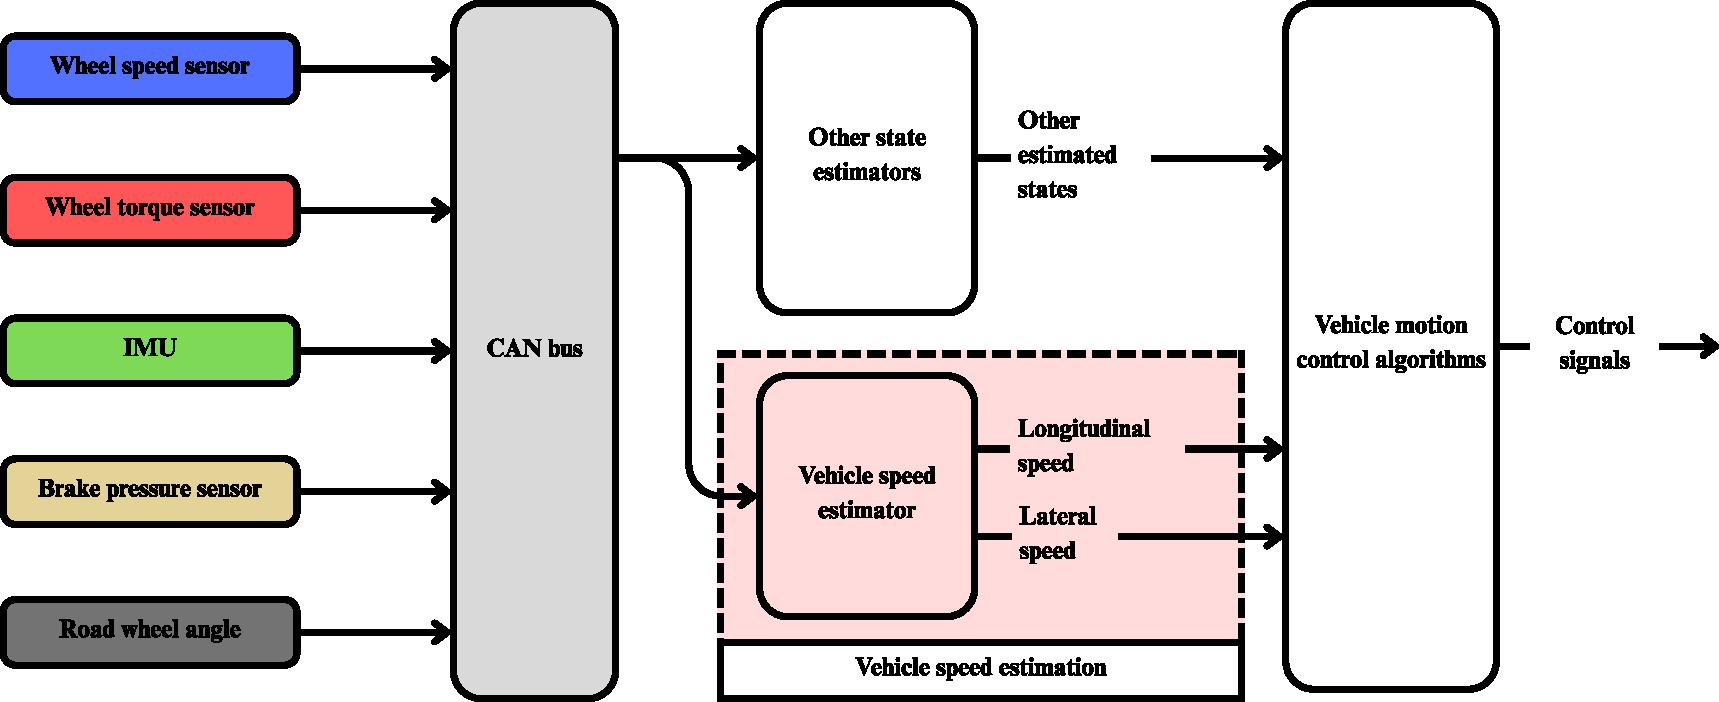
\includegraphics[width=1\textwidth]{images/Vehicle speed estimator.pdf}
    \caption{Vehicle speed estimation in the simplified control}
    \label{fig:vehicle speed estimation}
\end{figure}
\FloatBarrier

\subsection{Direct estimation}

When directly estimating any state of the vehicle, the structure is the following. The trained AI model receives the sensor data as inputs and outputs the state for which it was trained. In this thesis the state to estimate is the vehicle's longitudinal and lateral speed. 

The question now arises what models are suitable for this application? The possible models to use in this scenario are models that can handle time series data well and can estimate an output based on the sequence it was provided with. The possible models are the following:
\begin{itemize}
    \item Basic/simple Recurrent Neural Network (RNN)
    \item Long-short Term Memory (LSTM)
    \item Gated Recurrent Unit (GRU)
    \item Transformer for time series
    \item Temporal Convolutinal Network (TCN)
\end{itemize}

The teaching phase of these models will be relatively similar. All models will be taught on previously recorded sensor data coming from vehicle simulations and real-life vehicle tests. These recorder datasets will be extended with a longitudinal and lateral speed values calculated from the GNSS measurements. This way every input will be labeled with the desired output.

\subsection{Combination of existing estimators with AI model}

As it can be seen in the literature review that there are already existing applications of combining an AI model with an already established state estimator. The key advantages of this approach could be improved robustness, adaptive parameter tuning of the applied filter with implementing AI and non-linear error compensation.

Some possible implementations can be the following:
\begin{itemize}
    \item Residual learning:
    \begin{itemize}
        \item A neural network predicts the residual error from a standard Extended Kalman Filter (EKF) applied for vehicle speed estimation. The final speed will result from the combination of the estimated and the neural network's value for the residual. 
    \end{itemize}
    \item Neural network aided Kalman filter:
    \begin{itemize}
        \item The parts of the Kalman filter are replaced with trained modules
        \item E.g when the predict module is replaced by a neural network that determines the next state. 
    \end{itemize}
    \item Adaptive gain scheduler:
    \begin{itemize}
        \item The AI module dynamically tunes the noise covariance of the implemented Kalman filter based on the CAN signals. 
    \end{itemize}
\end{itemize}

\subsection{Advantages and disadvantages of AI application}

Prior to moving on to describing the developed models and estimators it is important to state the advantages and disadvantages when applying an AI model to a vehicle's control system. In case of a vehicle that is designed to be in contact (to transport or be driven by) with humans, the developed control system has to comply with specific international standards (e.g ISO 26262) that assures the safety of the system.

The main advantage when implementing AI to a vehicle control system is the possibility of capturing non-linear relationships between the CAN signals to estimate an arbitrary state. This property makes it possible to establish complex relationships between state variables without the knowledge of more complicated physical formulas. 

On the other hand, there are some disadvantages that need to be considered. An implemented AI can be considered as a black box where the inner operation makes it difficult to validate from safety relevant perspective. This also creates a part of the system that lacks transparency and explainability. An other disadvantage may arise from missing out on data quality and availability. Resource constraints in embedded systems may also block usability if the created model uses more computational power or memory than the available amount. 